\subsubsection{Volume Infused Loadcell Clamp Design}

The drawings below outline the fluid infusion loadcell clamp, two are required. Two of these can be fixed together on a stand to provide a clamp for the fluid infusion loadcell.
The four bolt and nut holes allow the two parts to be clamped together around the upright support. The internal nut hole and through bolt hole allow a single bolt ant nut to act as grub screw to fix the clamp to the upright support. The two through holes allow bolts to pass through the part to fix the loadcell to the clamp.


\begin{figure}[h]
    \centering
    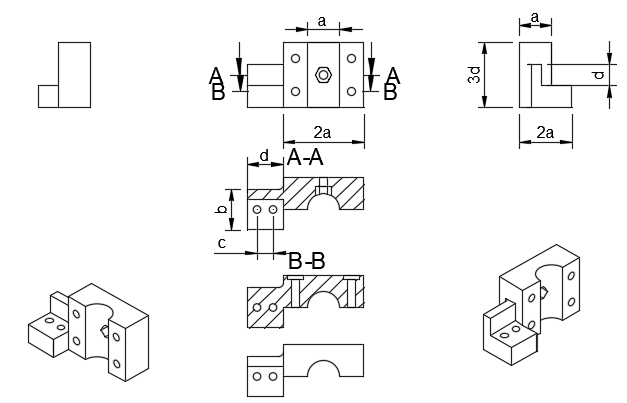
\includegraphics[width=0.7\textwidth]{Figures/SupportDrawings/vol_inf_loadcell_clamp_drawing.png}
    \caption{Volume Infused Loadcell Clamp Drawings}
    \label{fig:viloadcellclampdrawing}
  \end{figure}

\begin{enumerate}
  \item[a)] The diameter of the upright stand/trolley + \textgreater\ 4mm
  \item[b)] Twice the width of the loadcell + 4mm
  \item[c)] The distance between the centre points of the two tapped holes at each end of the loadcell
  \item[d)] Height of the loadcell
  \item[Nb.] Create holes to accommodate the chosen bolts
  \item[Nb.] Create hexagonal holes to accommodate the corresponding nuts, a tight fit makes it easier to move the bolts without the nuts dropping out
\end{enumerate}